% This is a comment.
% the region directly below this comment, up till the command \begin{document} is known as the 'preamble'
% basic setup
\documentclass{article}
\usepackage[english]{babel}
\usepackage[utf8]{inputenc}

% for mathematics
\usepackage{amsmath}
\usepackage{amsthm}
% define theorems, lemmas, etc
\newtheorem{theorem}{Theorem}
\newtheorem{lemma}{Lemma}
\newtheorem{corollary}{Corollary}
\newtheorem{definition}{Definition}
\newtheorem{example}{Example}
\usepackage{amssymb}

% for adjusting margins
\usepackage{geometry}
\geometry{
	a4paper,
 	left=26mm,
 	right=20mm,
 	top=33mm,
 	bottom=38mm
}

% for introducing urls
\usepackage{url}

% for colored text
\usepackage{color}

% for creating lists
\usepackage{enumerate}

% for import graphics
\usepackage{graphicx}

% include algorithm package
\usepackage[]{algorithm2e}

% change font to times new roman
%\usepackage{times}

% title details
\title{QF4102 Financial Modelling and Computation Assignment 1}
%\date{}
\author{G01 Wang Zexin, Chen Penghao}

%~~~~~~~~~~~~~~~~~~~~~~~~~~~~~~~~~~~~~~~~~~~~~~~~~~~~~~~~~~~~~~~~~~~~~~~~~~~~~~
\begin{document}

% insert title
\maketitle
% make a new page
\newpage

\section{Question 1}
\subsection*{\emph{Statement of the problem}}
Write a Matlab function for the exact solution of a European down-and-out call option. Your function must be able to \textbf{work with the initial underlier price $S_{0}$ in a vector form}.
\subsection{Data collection and preparation}
The business day chosen, day X is 28 Feb, 2017 within the 9-day period. The settlement prices of Eurodollar futures contracts which expire in March 2017, June 2017, September 2017, December 2017, March 2018, \dots , up to December 2026, (i.e. 10 years into the future) have been collected from the CME group website into the \emph{raw\_data} sheet of the excel file.\\
A screenshot of the webpage has been obtained and shown below.
\begin{figure}[h]
  \centering
  \begin{minipage}[h]{0.32\textwidth}
    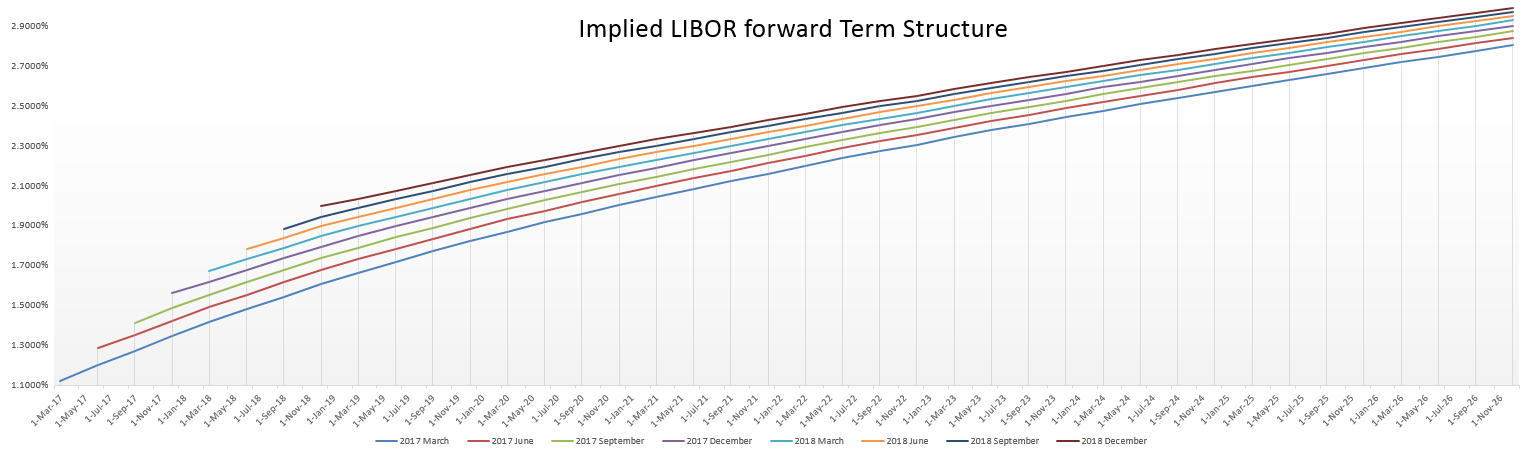
\includegraphics[width=\textwidth]{biu.PNG}
  \end{minipage}
  \hfill
  \begin{minipage}[h]{0.32\textwidth}
    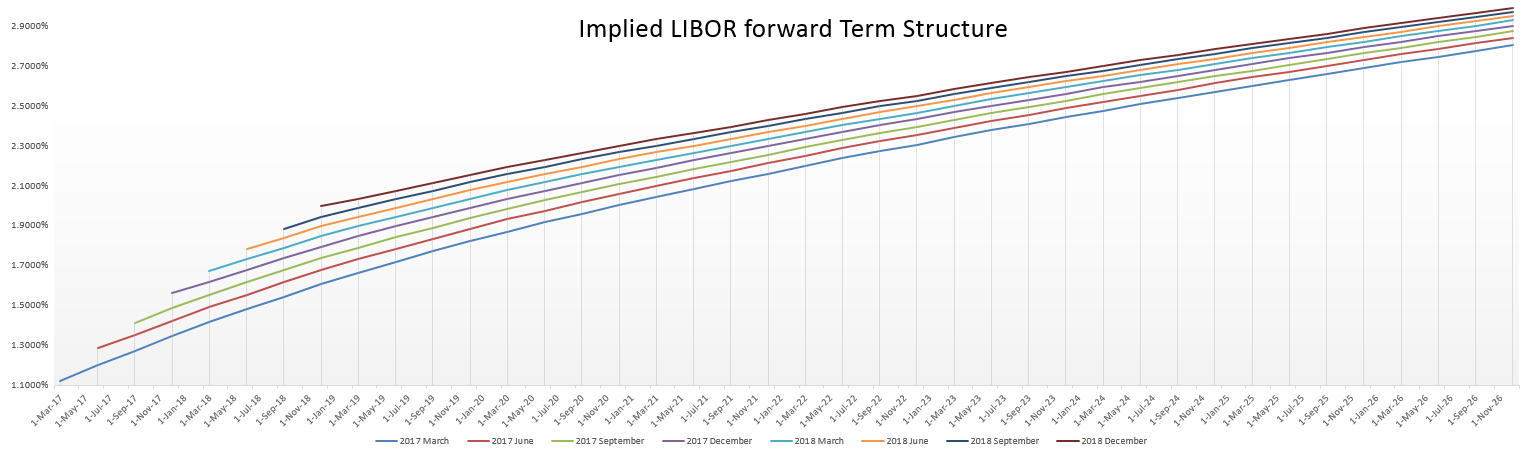
\includegraphics[width=\textwidth]{biu.PNG}
  \end{minipage}
  \hfill
  \begin{minipage}[h]{0.32\textwidth}
    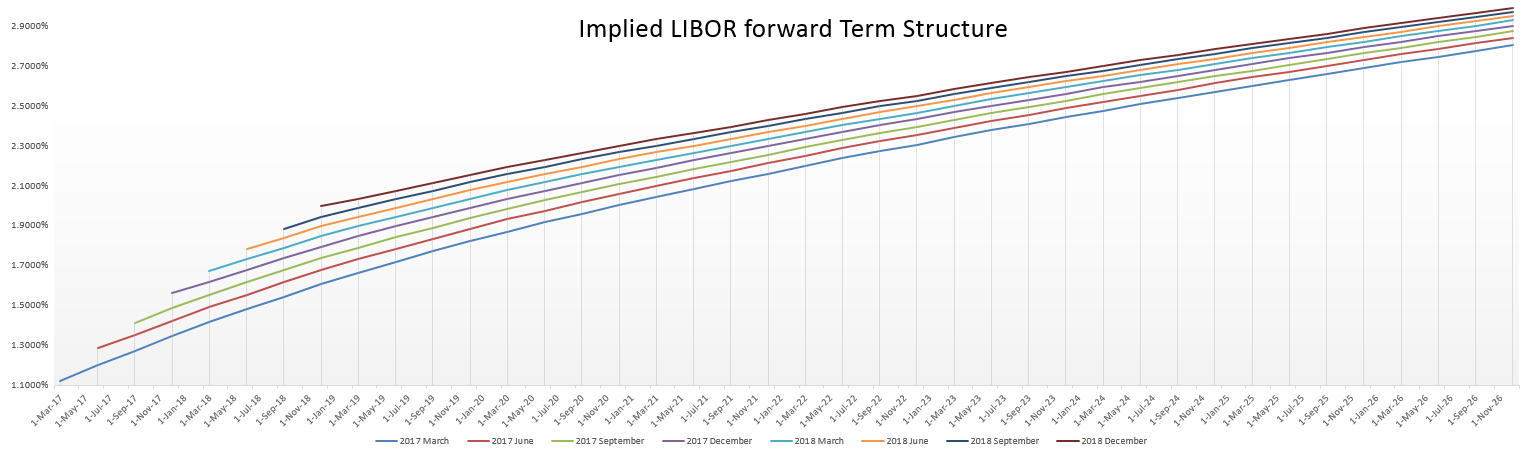
\includegraphics[width=\textwidth]{biu.PNG}
  \end{minipage}
	\caption{Screenshot of the webpage showing settlement prices of ED futures}
\end{figure}

Also, the expiry dates can be obtained from the CME group website. A sheet of the settlement dates have been collected into the \emph{raw\_dates} sheet of the excel file. A screenshot of the webpage has been obtained and shown below.
\begin{figure}[h]
	\centering
	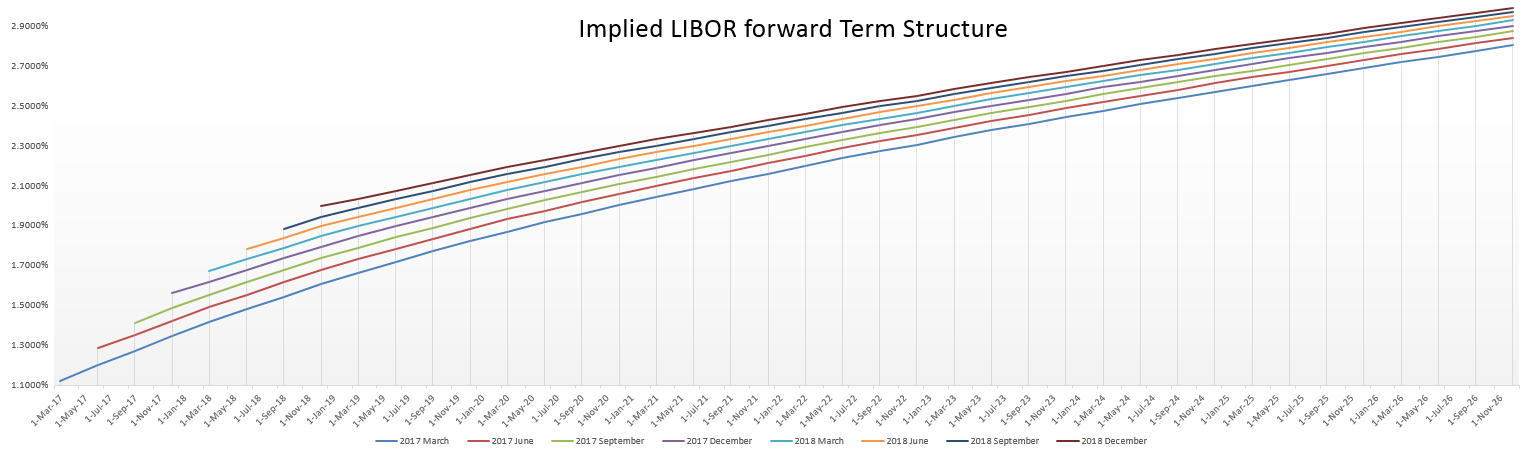
\includegraphics[scale=0.5]{biu.PNG}
	\caption{Screenshot of the webpage showing settlement dates of ED futures}
\end{figure}
\newpage

\subsection{Implied Forward LIBOR term structure}
As the index prices of Eurodollar futures have linear relationship with the implied forward 3-month LIBOR rate starting from the expiry dates of the Eurodollar futures until maturity of the Eurodollar time deposits, we are able to work out the implied forward 3-month LIBOR rates.\\[4mm]
Denote the forward rate from expiry date of the first futures to the $n$-th Eurodollar futures by $f_{n}$, numbers of days until maturity of the underlying of the $i$-th Eurodollar futures by $m_{i}$, implied 3-month LIBOR rate of the underlying of the $i$-th Eurodollar futures by $l_{i}$ and the settlement price of the $i$-th Eurodollar futures by $P_{i}$.\\[4mm]
$$1 + \frac{\sum_{i=1}^{n} m_{i}}{360}f_{n} = [\prod_{i=1}^{n} (1 + l_{i}\frac{m_{i}}{360}) - 1] \frac{\sum_{i=1}^{n} m_{i}}{360}$$
\begin{equation}
\begin{split}
f_{n} &= [\prod_{i=1}^{n} (1 + l_{i}\frac{m_{i}}{360}) - 1] \frac{360}{\sum_{i=1}^{n} m_{i}}\\
&= [\prod_{i=1}^{n} (1 + \frac{100 - P_{i}}{100}\frac{m_{i}}{360}) - 1] \frac{360}{\sum_{i=1}^{n} m_{i}}
\end{split}
\end{equation}
\\[4mm]
\begin{figure}[h]
	\centering
	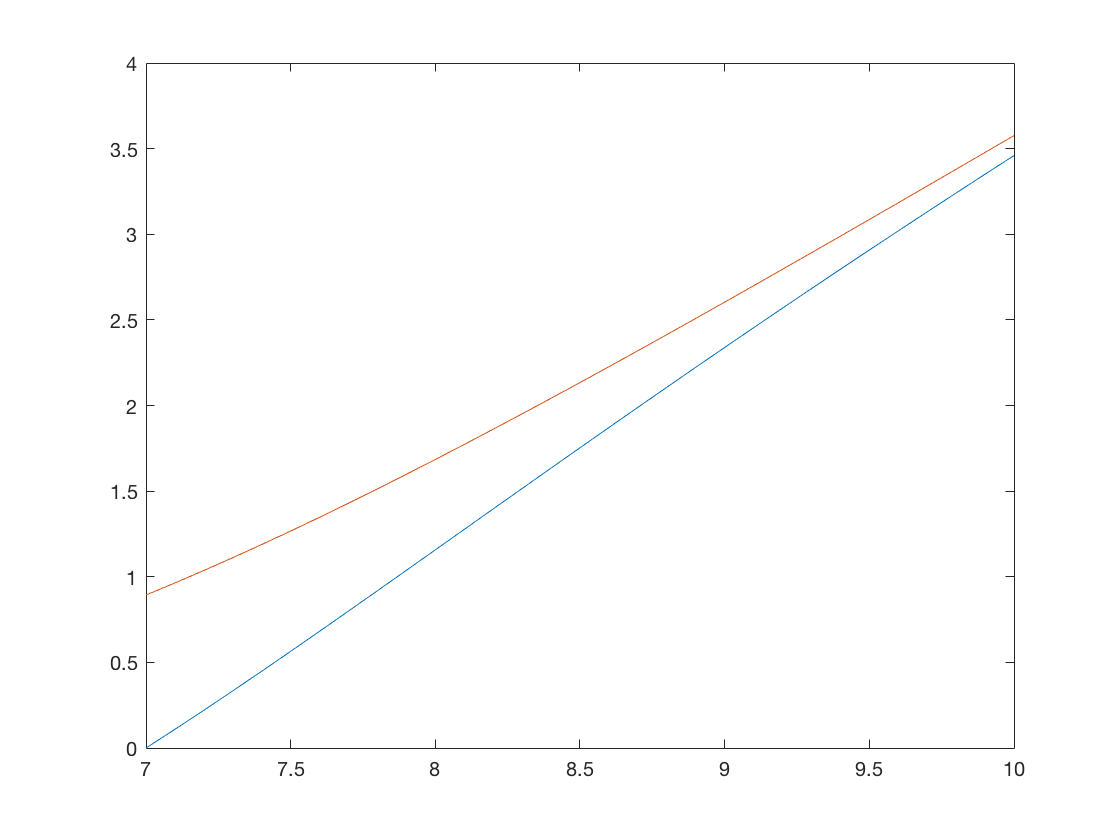
\includegraphics[scale=0.3]{A1_1_plot.png}
	\caption{Prices of down-and-out and vanilla call option against current underlying price}
\end{figure}
\\[2mm]
\newpage

\subsection{Swap Rate for Deferred Interest Rate Swap}
Similar to the previous section, we can work out forward term structure from the index prices of Eurodollar futures. The discount factors can be computed using the forward rates. The swap rate for deferred interest rate swap is simply the swap rate for the expected forward rates, as specified in equation (2).
\\Denote the discount factor from time 0 to $K$-th year by $d_{0,K}$, the forward rate (not annualized) from time 0 to the $i$-th year by $f_{i}$, and the swap rate by $r$.
\begin{equation}
\begin{split}
r &= \frac{1 - d_{0,K}}{\sum_{i=1}^{K} d_{0,i}}\\
&= \frac{1 - (1 + f_{K})^{-1}}{\sum_{i=1}^{K} (1 + f_{i})^{-1}}
\end{split}
\end{equation}
\\Tabulated series of deferred swap rates starting from the March, June, September and December of 2017 with maturity of 1, 2, \dots, 9 years are displayed in Figure 5:
\\Also, other than the illustrative use of the \emph{GetSwapRate} function in the excel sheets, the diagram of the deferred interest swap rates can be plotted.
\begin{figure}[h]
	\centering
	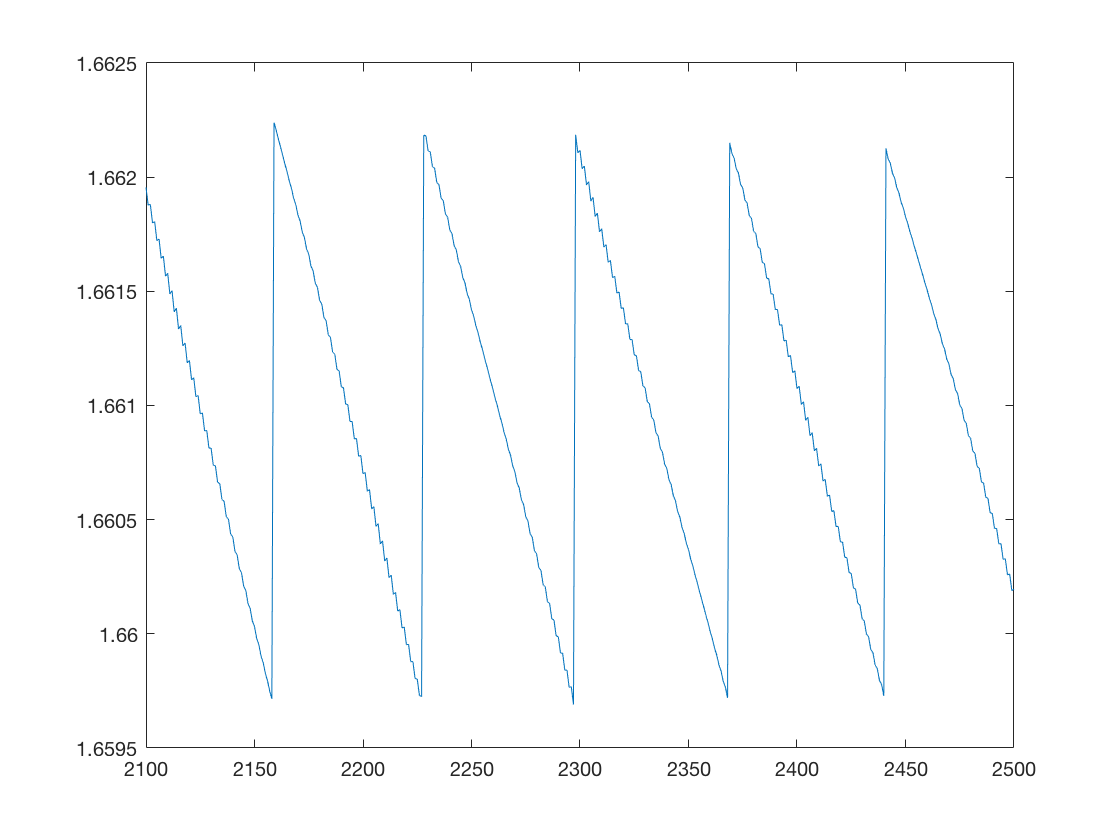
\includegraphics[scale=0.3]{A1_1_plot2.PNG}
	\caption{Prices of European down-and-out call against number of time intervals}
\end{figure}
\\We shall observe that the calculated deferred swap rates are rational, as the curvature of the upward curve is convex.
\newpage

\section{Efficient Stock Portfolios}
\subsection*{Statement of the problem}
Write a Matlab function that implements version 1 of the single-state variable binomial tree method for approximating prices of a European floating strike lookback put option (newly issued) with $0.5$ year to maturity, current underlying price of \$1, volatility of $40\%$, dividend yield of $2\%$ and risk free rate of $4\%$. Obtain option value estiamtes for number of time steps $N$ being $200$ to $20000$ in increments of $200$. Obtain a graph of these option values versus $N$.\\
Write also a Matlab function to price European floating strike lookback put option (not newly issued). Test with same parameters with running max of \$$1.3$.

\subsection{Newly issued European floating strike lookback put options}
For the floating strike type of lookback options, we can change from a two-state model to single-state model. We make use of this property $V(A_{t},S_{t},t) = S_{t}V(\frac{A_{t}}{S_{t}}, 1, t)$, and use the new symbol $x_{t} = \ln(\frac{A_{t}}{S_{t}})$ to represent the current state on the binomial tree. Value of the option can thus be represented by $W(x_{t}, t) = \frac{V(exp(x_{t}), 1, t)}{S_{t}}$.\\
Since in this case we are only interested in the $A_{t}$ being the maximum value of underlying over time, the binomial updates of $A_{t}$ can be simplied as:
\begin{equation}
  A_{t}=
  \begin{cases}
    A_{t-1}, & \text{if}\ S_{t} = dS_{t-1} \\
    \max(A_{t-1}, S_{t}), & \text{otherwise}
  \end{cases}
\end{equation}
Furthermore, we use this upon the binomial updates of $x_{t}$:
\begin{equation}
  x_{n}^{k}=
  \begin{cases}
    x_{n-1}^{\frac{k+1}{2}} + {^{\Delta}x}, & \text{if}\ k \text{ is odd} \\
    \max(x_{n-1}^{\frac{k}{2}} - {^{\Delta}x}, 0), & \text{otherwise}
  \end{cases}
\end{equation}
where ${^{\Delta}x} = \sigma \sqrt{^{\Delta}t}$
The binomial update equation for $W(x_{n}^{k}, t_{n})$ is:
$$ W(x_{n}^{k}, t_{n}) = \exp(-r{^{\Delta}t})[puW(x_{n+1}^{2k}, t_{n+1}) + (1-p)dW(x_{n+1}^{2k+1}, t_{n+1})] $$
\begin{algorithm}[H]
 \KwData{$r, \sigma, S_{0}, \tau, N, q$}
 \KwResult{$p_{0}$, Option Premium}
 Initialization\;
 $N = \frac{T}{\delta t}$\;
 $x_{n}^{k} = k{^{\Delta}x}$\;
 Set the boundary conditions\;
 \For {i = $\max(j-N, 0)$ \dots $j+N+1$} {
  $W_{N}^{i} = \exp(x_{N}^{i}) - 1$\;
 }
 \For {n = N-1, N-2, \dots 0} {
  \If {$j - n \le 0$} {
    $W_{n}^{0} = exp(-r{^{\Delta}t})[puW_{n+1}^{0}+(1-p)dW_{n+1}^{1}]$\;
  }
  \For {k = $\max(j-n,1), \dots, j + n + 1$} {
    $W_{n}^{k} = exp(-r{^{\Delta}t})[puW_{n+1}^{k-1}+(1-p)dW_{n+1}^{k+1}]$\;
  }
 }
 $p_{0} = S_{0}W_{0}^{0}$\;
\caption{Algorithm for pricing newly issued floating strike lookback put}
\end{algorithm}
\newpage

\subsection{Not newly issued European floating strike lookback put options}
In the previous case we could take advantage of the characteristic of lookback option in which all the maximum values correspond to the potential stock prices in the binomial tree. However in this case, since the option is not newly issued and we may have a previous running max which does not correspond to any of the potential stock prices, we cannot use the single state variable to fully represent both the current stock price and the running max. Therefore the following adjustment is needed:
\begin{itemize}
	\item Compare $\tilde{A}$ and $S_{0}$, if $\tilde{A}$ is smaller, treat this like a newly issued lookback option and use the previous case's algorithm
	\item let $x_{0} = \ln \frac{\tilde{A}}{S_{0}}$
	\item Determine for an integer $j$ such that $j{^{\Delta}x} < x_{0} < (j+1){^{\Delta}x}$
	\item Grow two separate linear trees from $x_{0}^{j}$ and $x_{0}^{j+1}$
	\item Perform the backward time binomial updates
	\item Interpolate between two option values at the roots to obtain option premium
\end{itemize}
Below is an algorithm developed based on this idea:\\
\begin{algorithm}[H]
 \KwData{$r, \sigma, S_{0}, \tau, N, q, \tilde{A}$}
 \KwResult{$p_{0}$, Option Premium}
 Initialization\;
 let $x_{0} = \ln \frac{\tilde{A}}{S_{0}}$ be the initial  of the single state\;
 Choose integer $j$ such that $j{^{\Delta}x} < x_{0} < (j+1){^{\Delta}x}$\;
 $N = \frac{T}{\delta t}$\;
 Set the boundary conditions\;
 \For {i = $\max(j-N, 0)$ \dots $j+N+1$} {
  $W_{N}^{i} = \exp(x_{N}^{i}) - 1$\;
 }
 \For {n = N-1, N-2, \dots 0} {
  \If {$j - n \le 0$} {
    $W_{n}^{0} = exp(-r{^{\Delta}t})[puW_{n+1}^{0}+(1-p)dW_{n+1}^{1}]$\;
  }
  \For {k = $\max(j-n,1), \dots, j + n + 1$} {
    $W_{n}^{k} = exp(-r{^{\Delta}t})[puW_{n+1}^{k-1}+(1-p)dW_{n+1}^{k+1}]$\;
  }
 }
 $p_{0}$ is approximated by interpolating between $S_{0}W_{0}^{j}$ and $S_{0}W_{0}^{j+1}$\;
\caption{Algorithm for pricing not newly issued floating strike lookback put}
\end{algorithm}
\newpage

\subsection{Analyze, compare and comment on the results}
\begin{figure}[h]
	\centering
	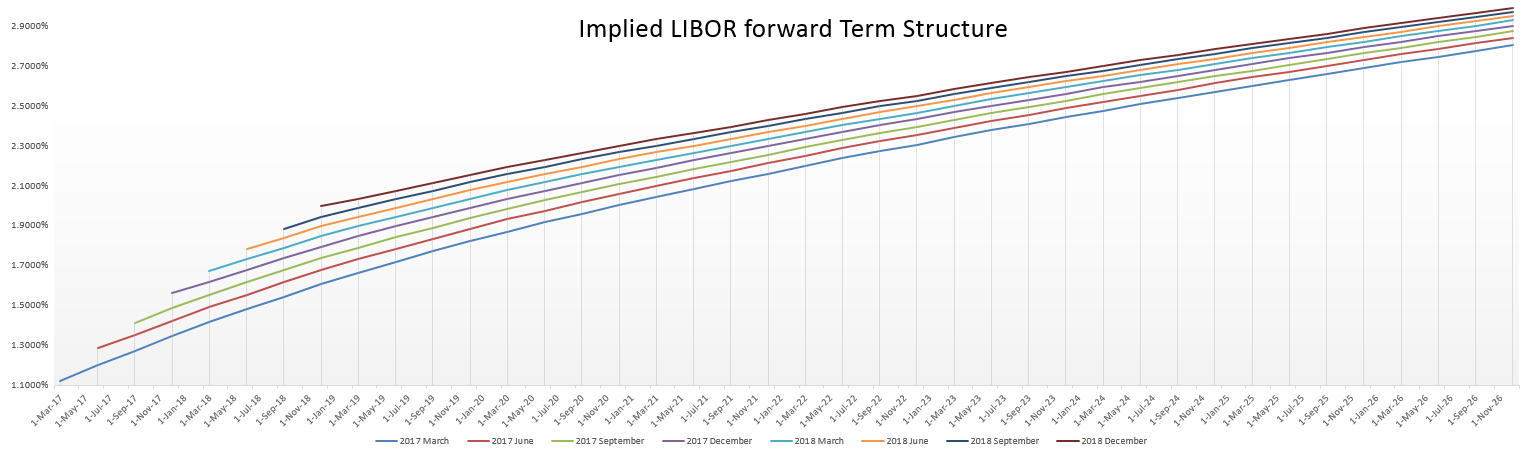
\includegraphics[scale=0.4]{biu.PNG}
	\caption{Prices of newly issued floating strike lookback put against the number of time intervals}
\end{figure}
From Figure 6, we can easily observe that as the number of time intervals used in the binomial tree method slowly increases from $200$ to $20000$, the prices obtained for the newly issued floating strike lookback put option monotonically increases from $0.226$ to $0.236$. The rate of increase gradually drops as the price increases, and we see this as an indication that the price obtained is converging to the true value of the option.\\[4mm]
If the true value is actually around $0.236$, we should be confident that the binomial tree method with single-state modification for the European floating strike lookback put option can almost always give a good estimate of the price since the initially computed price with only $200$ time interval is very close to the true value. However, the closed-form formula does not exist for this case but once we have the finite different equations for the lookback options, the prices from FDM can be used to cross-validate the ones from binomial tree methods.\\[4mm]
A natural question to ask may be : why are stocks like XOM, GS and FDX still kept within the portfolio? Perhaps it will be more rational if we leave these stocks out, as the weights suggested that these stocks are not preferred over other stocks in the Capital Asset Pricing Model. One simple rationale may answer this: when gold as a commodity for trading has generally lower return compared to stocks, people will still tend to hold gold as a means to hedge against the Equity Market risks. Similar to the gold case, although these stocks may not generate good returns, inclusion of them into the portfolio can help to diversify the risks and effectively reduce portfolio variance.\\[4mm]
\begin{figure}[h]
	\centering
	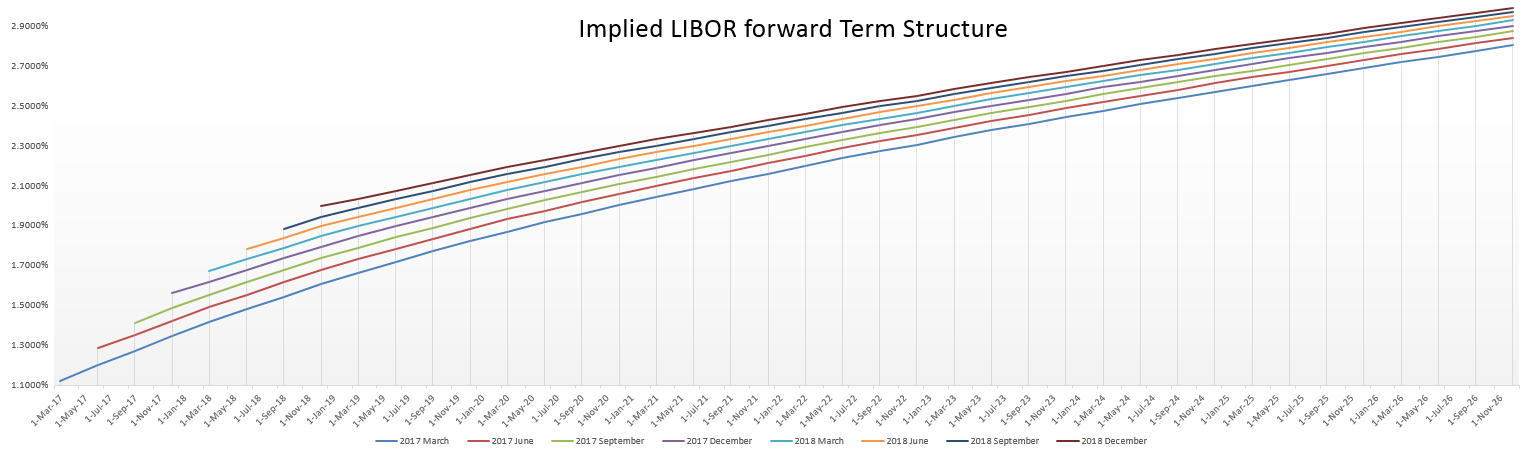
\includegraphics[scale=0.4]{biu.PNG}
	\caption{Prices of not newly issued floating strike lookback put against the number of time intervals}
\end{figure}
Surely, another argument may follow up: among this basket of stocks, when more people are holding NVS and shorting GS, the stock price of NVS will increase and its return will go lower, while stock price of GS will decrease and its return will go higher. In this sense, the return of NVS and GS will become more negatively correlated. From the point of view of an investor, he/she will not choose to long one and short another in the same time, in order to reduce the covariance. Hence, we can conclude that, given in a relatively rational market with rational market adjustments done by the investing activities, we expect to see portfolio managers rebalancing their portfolios quite often. This argument is also valid for the content in our last lecture on \emph{VaR} as the covariance matrix for Basel calculation is required to be updated at least quarterly.
\begin{figure}[h]
	\centering
	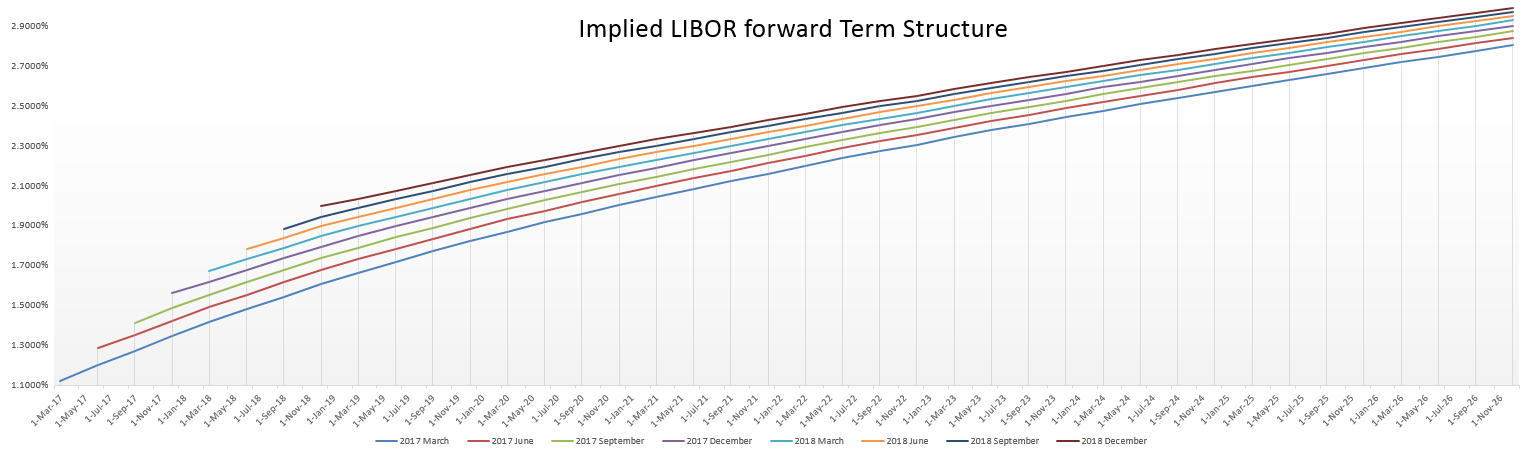
\includegraphics[scale=0.5]{biu.PNG}
	\caption{$\sigma-\bar{r}$ diagram of 100 points}
\end{figure}
\\[4mm]Also, since it may be difficult to directly observe the efficient frontier from only 25 points, I have plotted a $\sigma-\bar{r}$ diagram with 100 points on the efficient frontier by incrementing $\lambda$ at 0.01 only. From the diagram with more points from the efficient frontier, we can see that the slope of the frontier decreases at a decreasing rate, and eventually becomes one straight line. This shows the existence of asymptote of the efficient frontier.
\begin{figure}[h]
  \centering
  \begin{minipage}[h]{0.85\textwidth}
    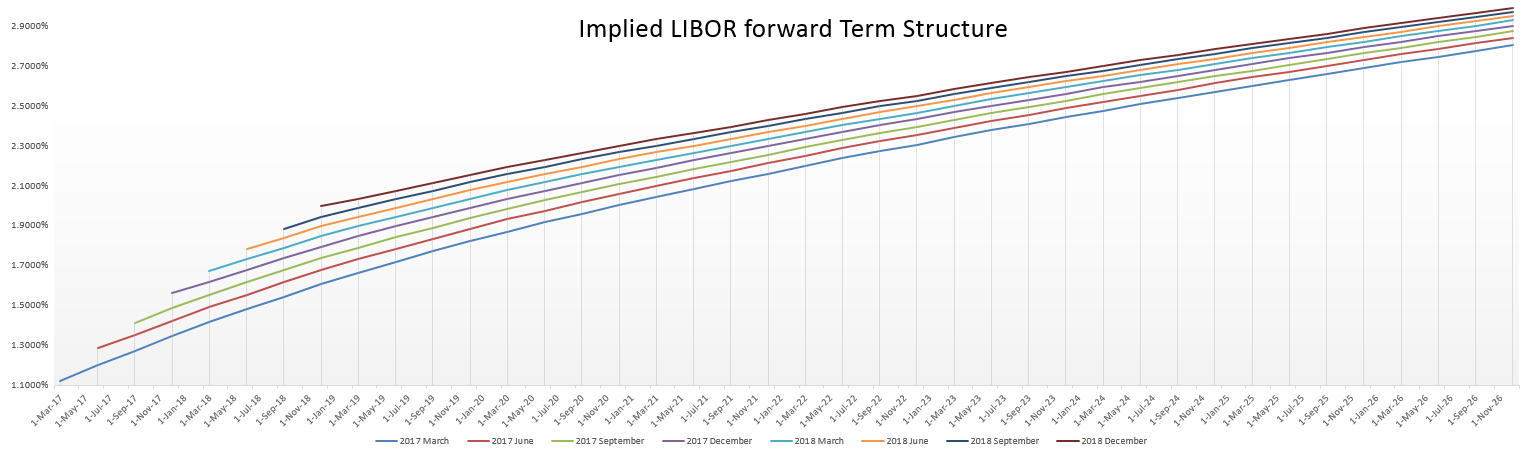
\includegraphics[width=\textwidth]{biu.PNG}
  \end{minipage}
  \hfill
  \begin{minipage}[h]{0.1\textwidth}
    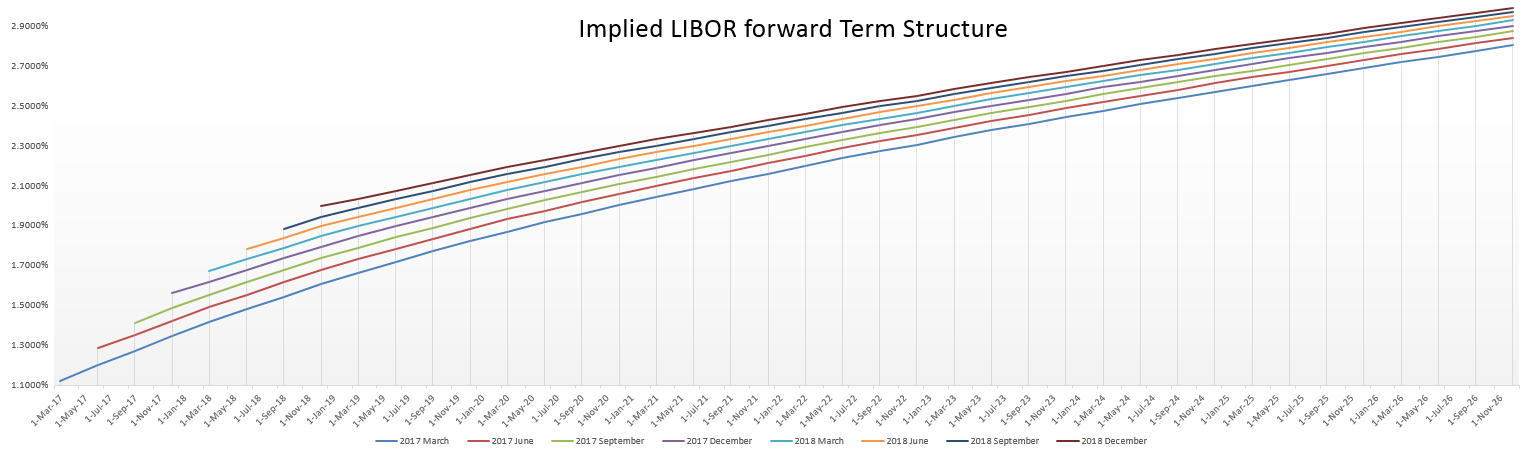
\includegraphics[width=\textwidth]{biu.PNG}
  \end{minipage}
  \caption{Template to plot graphs side by side}
\end{figure}
\end{document}